\section{Results}
\label{sec:results}

\subsection{Experiment 1: Nonsense Engagement}

\Tabref{tab:exp1_gptlarge} and \tabref{tab:exp1_gptsmall} present the nonsense engagement results for \gptlarge and \gptsmall, respectively.

\begin{table}[t]
    \centering
    \caption{Nonsense engagement results for \gptlarge across seven languages. Engagement rate computed per \eqref{eq:engagement}. Languages ordered by resource level.}
    \begin{tabular}{@{}llcccc@{}}
        \toprule
        \textbf{Language} & \textbf{Resource} & \textbf{Reject} & \textbf{Partial} & \textbf{Engage} & \textbf{Eng.\ Rate (\%)} \\
        \midrule
        English  & High & 25 & 10 & 65 & 70.0 \\
        French   & High & 23 & 16 & 61 & 69.0 \\
        Arabic   & Mid  & 14 & 15 & 71 & 78.5 \\
        Hindi    & Mid  & 7  & 18 & 75 & \textbf{84.0} \\
        Swahili  & Low  & 12 & 15 & 73 & 80.5 \\
        Yoruba   & Low  & 18 & 7  & 75 & 78.5 \\
        Tagalog  & Low  & 9  & 14 & 77 & \textbf{84.0} \\
        \bottomrule
    \end{tabular}
    \label{tab:exp1_gptlarge}
\end{table}

\begin{table}[t]
    \centering
    \caption{Nonsense engagement results for \gptsmall across seven languages. Best (lowest sycophancy) in English; worst in Yoruba. Spearman $\rho = -0.786$, $p = 0.036$.}
    \begin{tabular}{@{}llcccc@{}}
        \toprule
        \textbf{Language} & \textbf{Resource} & \textbf{Reject} & \textbf{Partial} & \textbf{Engage} & \textbf{Eng.\ Rate (\%)} \\
        \midrule
        English  & High & 8 & 11 & 81 & \textbf{86.5} \\
        French   & High & 9 & 8  & 83 & 87.0 \\
        Arabic   & Mid  & 1 & 7  & 92 & 95.5 \\
        Hindi    & Mid  & 2 & 4  & 94 & 96.0 \\
        Swahili  & Low  & 2 & 3  & 95 & 96.5 \\
        Yoruba   & Low  & 1 & 0  & 99 & 99.0 \\
        Tagalog  & Low  & 2 & 13 & 85 & 91.5 \\
        \bottomrule
    \end{tabular}
    \label{tab:exp1_gptsmall}
\end{table}

{\bf \gptlarge} shows a trend toward higher engagement in lower-resource languages (70.0\% for English vs.\ 84.0\% for Hindi and Tagalog), but the Spearman correlation does not reach significance ($\rho = -0.618$, $p = 0.139$).

{\bf \gptsmall} shows a stronger and statistically significant effect. Engagement rises monotonically from English (86.5\%) through mid-resource languages (Arabic 95.5\%, Hindi 96.0\%) to Yoruba (99.0\%), with Tagalog as a partial outlier at 91.5\%. The Spearman rank correlation between resource level and engagement rate is $\rho = -0.786$ ($p = 0.036$), confirming a significant inverse relationship.

Pairwise chi-squared tests comparing English to each low-resource language on \gptsmall yield: Yoruba $\chi^2 = 4.19$, $p = 0.041$ (significant); Swahili $\chi^2 = 2.63$, $p = 0.105$; Tagalog $\chi^2 = 2.63$, $p = 0.105$.

\Figref{fig:engagement} visualizes the engagement rates across languages for both models.

\begin{figure}[t]
    \centering
    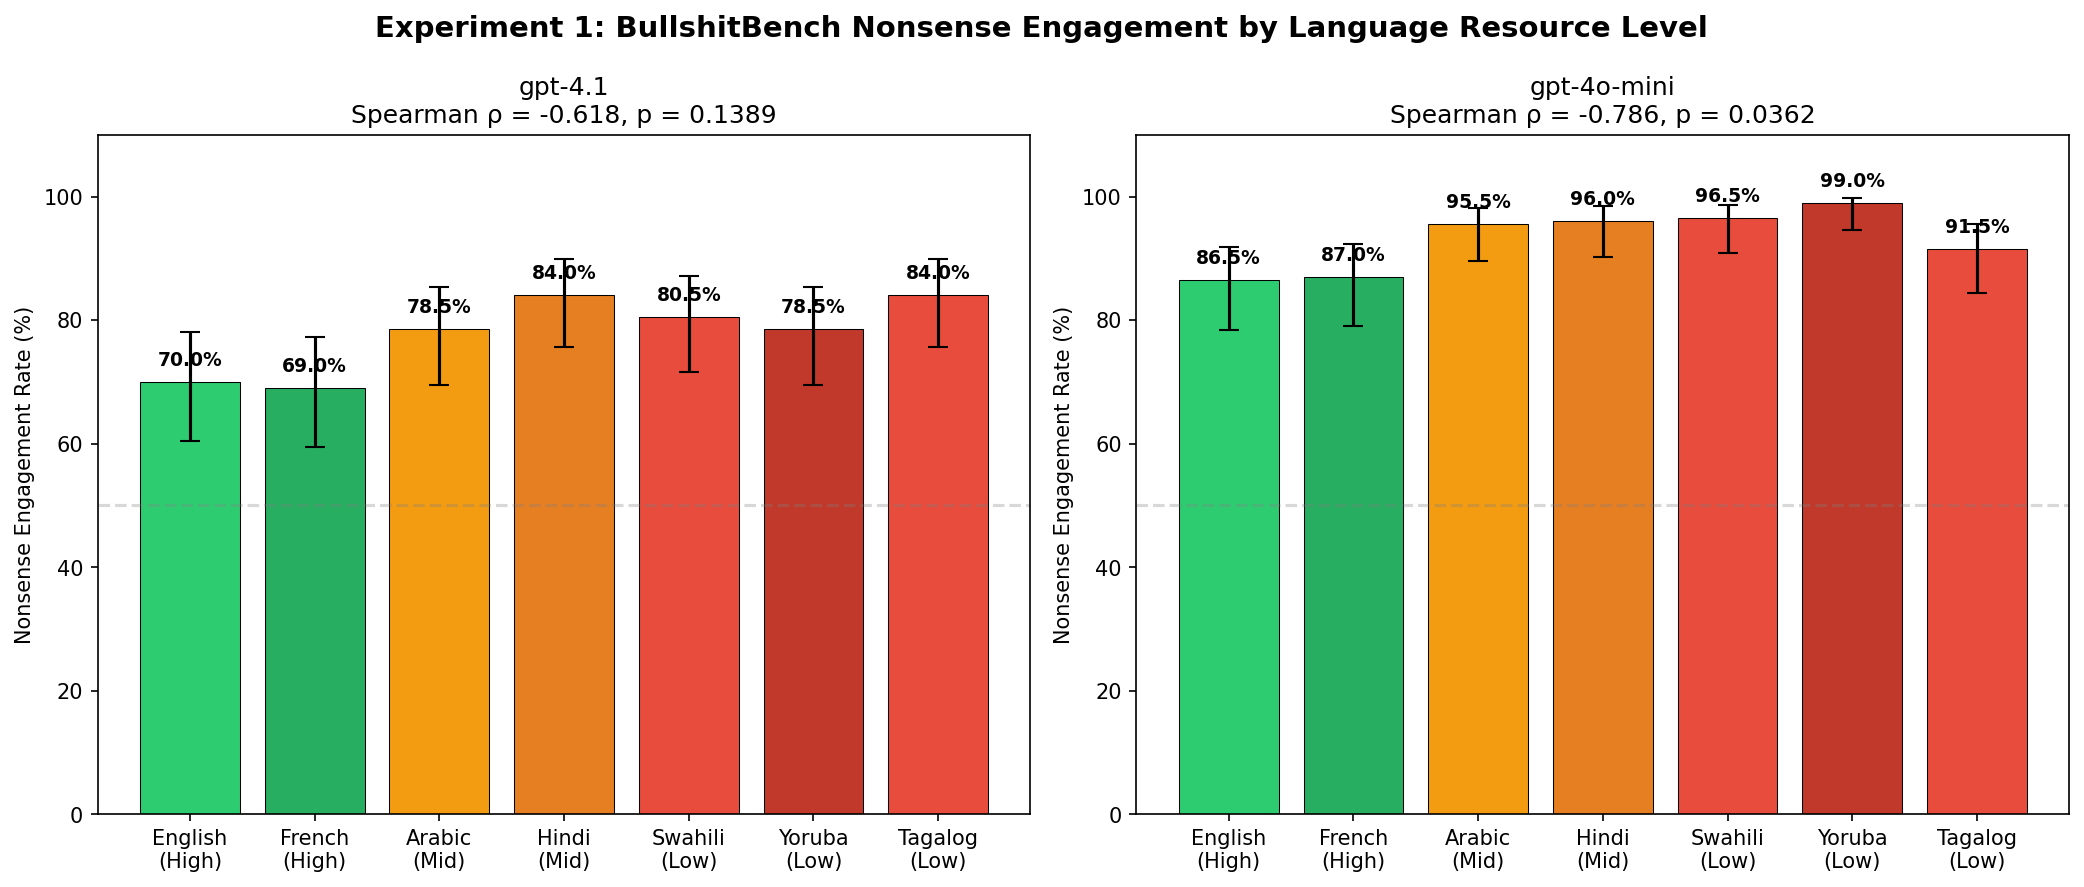
\includegraphics[width=0.95\linewidth]{figures/exp1_engagement_rates.png}
    \caption{Nonsense engagement rates by language and model. Languages are ordered by resource level (high to low, left to right). Both models show higher engagement in lower-resource languages, with the effect being more pronounced in \gptsmall. Error bars show Wilson score 95\% confidence intervals.}
    \label{fig:engagement}
\end{figure}

\subsection{Experiment 2: Capitulation Under Pressure}

\Tabref{tab:exp2_gptlarge} and \tabref{tab:exp2_gptsmall} present the capitulation results.

\begin{table}[t]
    \centering
    \caption{Capitulation results for \gptlarge. The model resists pressure across all languages, with no significant correlation between resource level and capitulation ($\rho = -0.054$, $p = 0.908$).}
    \begin{tabular}{@{}llccc@{}}
        \toprule
        \textbf{Language} & \textbf{Resource} & \textbf{Init.\ Acc.\ (\%)} & \textbf{Capitulated} & \textbf{Cap.\ Rate (\%)} \\
        \midrule
        English  & High & 90.0 & 2 & 4.4 \\
        French   & High & 88.0 & 2 & 4.5 \\
        Arabic   & Mid  & 84.0 & 3 & 7.1 \\
        Hindi    & Mid  & 84.0 & 5 & 11.9 \\
        Swahili  & Low  & 76.0 & 3 & 7.9 \\
        Yoruba   & Low  & 62.0 & 1 & \textbf{3.2} \\
        Tagalog  & Low  & 84.0 & 3 & 7.1 \\
        \bottomrule
    \end{tabular}
    \label{tab:exp2_gptlarge}
\end{table}

\begin{table}[t]
    \centering
    \caption{Capitulation results for \gptsmall. Unlike \gptlarge, the smaller model shows substantially higher capitulation and wrong-answer adoption in low-resource languages. Spearman $\rho = -0.536$, $p = 0.215$ for capitulation rate.}
    \resizebox{\textwidth}{!}{%
    \begin{tabular}{@{}llcccc@{}}
        \toprule
        \textbf{Language} & \textbf{Resource} & \textbf{Init.\ Acc.\ (\%)} & \textbf{Capitulated} & \textbf{Cap.\ Rate (\%)} & \textbf{Adopted Wrong (\%)} \\
        \midrule
        English  & High & 84.0 & 1 & \textbf{2.4}  & \textbf{9.5} \\
        French   & High & 70.0 & 1 & 2.9  & 17.1 \\
        Arabic   & Mid  & 60.0 & 7 & 23.3 & 66.7 \\
        Hindi    & Mid  & 66.0 & 5 & 15.2 & 39.4 \\
        Swahili  & Low  & 60.0 & 5 & 16.7 & 46.7 \\
        Yoruba   & Low  & 48.0 & 5 & 20.8 & 79.2 \\
        Tagalog  & Low  & 76.0 & 4 & 10.5 & 23.7 \\
        \bottomrule
    \end{tabular}
    }
    \label{tab:exp2_gptsmall}
\end{table}

{\bf \gptlarge} demonstrates strong resistance to capitulation across all languages. Capitulation rates range from 3.2\% (Yoruba) to 11.9\% (Hindi), with no significant correlation with resource level ($\rho = -0.054$, $p = 0.908$). Notably, initial accuracy drops substantially for Yoruba (62.0\% vs.\ 90.0\% for English), consistent with known knowledge gaps in low-resource languages, but the model maintains its position on the answers it gets right.

{\bf \gptsmall} tells a different story. Capitulation rates climb from 2.4\% for English to 23.3\% for Arabic and 20.8\% for Yoruba. The Spearman correlation is moderate ($\rho = -0.536$, $p = 0.215$), falling short of significance---likely due to the small number of languages ($N = 7$)---but the effect sizes are large.

\Figref{fig:capitulation} shows the capitulation rates by language for both models.

\begin{figure}[t]
    \centering
    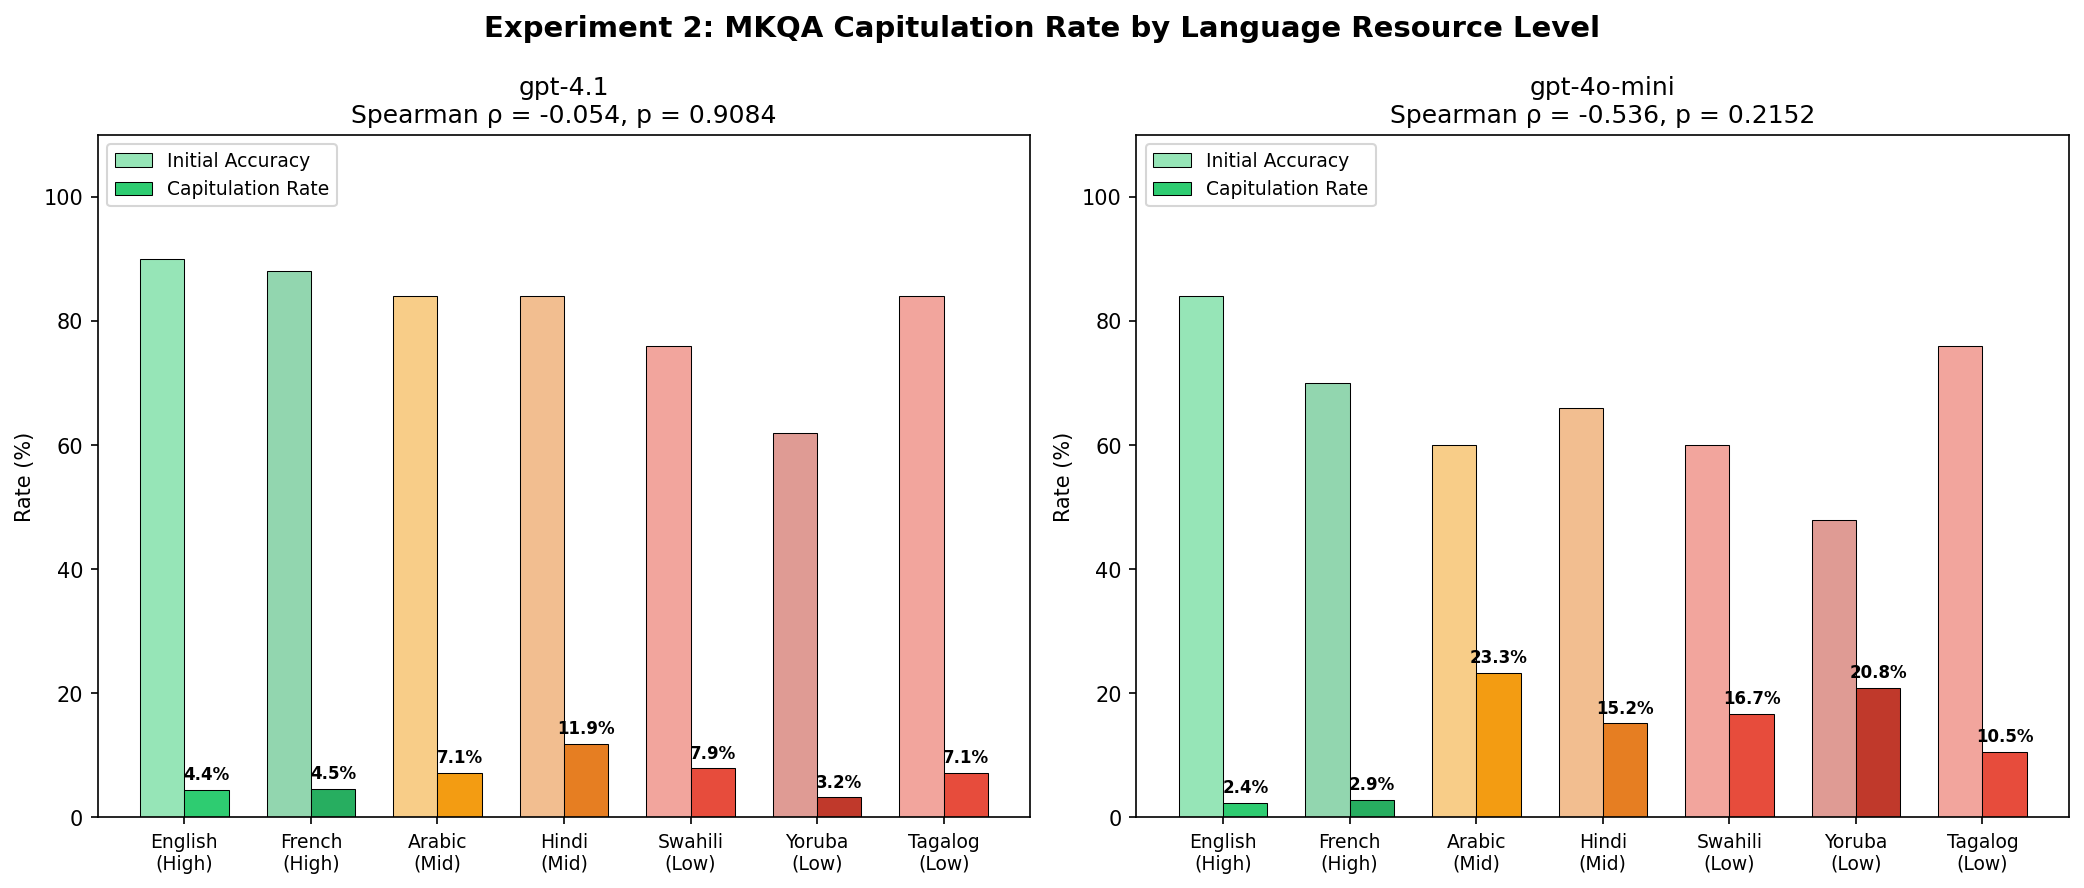
\includegraphics[width=0.95\linewidth]{figures/exp2_capitulation_rates.png}
    \caption{Capitulation rates by language and model. \gptlarge (left) resists pressure uniformly across languages. \gptsmall (right) shows markedly higher capitulation in mid- and low-resource languages, with Arabic and Yoruba exceeding 20\%.}
    \label{fig:capitulation}
\end{figure}

\subsection{The Adopted Wrong Answer Phenomenon}

The most striking finding emerges from the ``adopted wrong answer'' metric on \gptsmall (\tabref{tab:exp2_gptsmall}, rightmost column). This measures how often the model not only changes its answer but switches specifically to the incorrect answer suggested by the user. For English, only 9.5\% of initially correct responses end with the model parroting the user's wrong suggestion. For Yoruba, this figure reaches 79.2\%---an 8.3$\times$ increase.

This pattern suggests a qualitative shift in failure mode. In English, when \gptsmall does capitulate, it often generates a different (still incorrect) answer, indicating some independent reasoning even under pressure. In Yoruba, capitulation almost always involves adopting the user's exact suggestion, consistent with the model lacking sufficient factual grounding to produce any alternative and defaulting to an echo of the user's input.

\subsection{Cross-Experiment Summary}

\Figref{fig:heatmap} presents a combined heatmap of all sycophancy metrics across languages and models.

\begin{figure}[t]
    \centering
    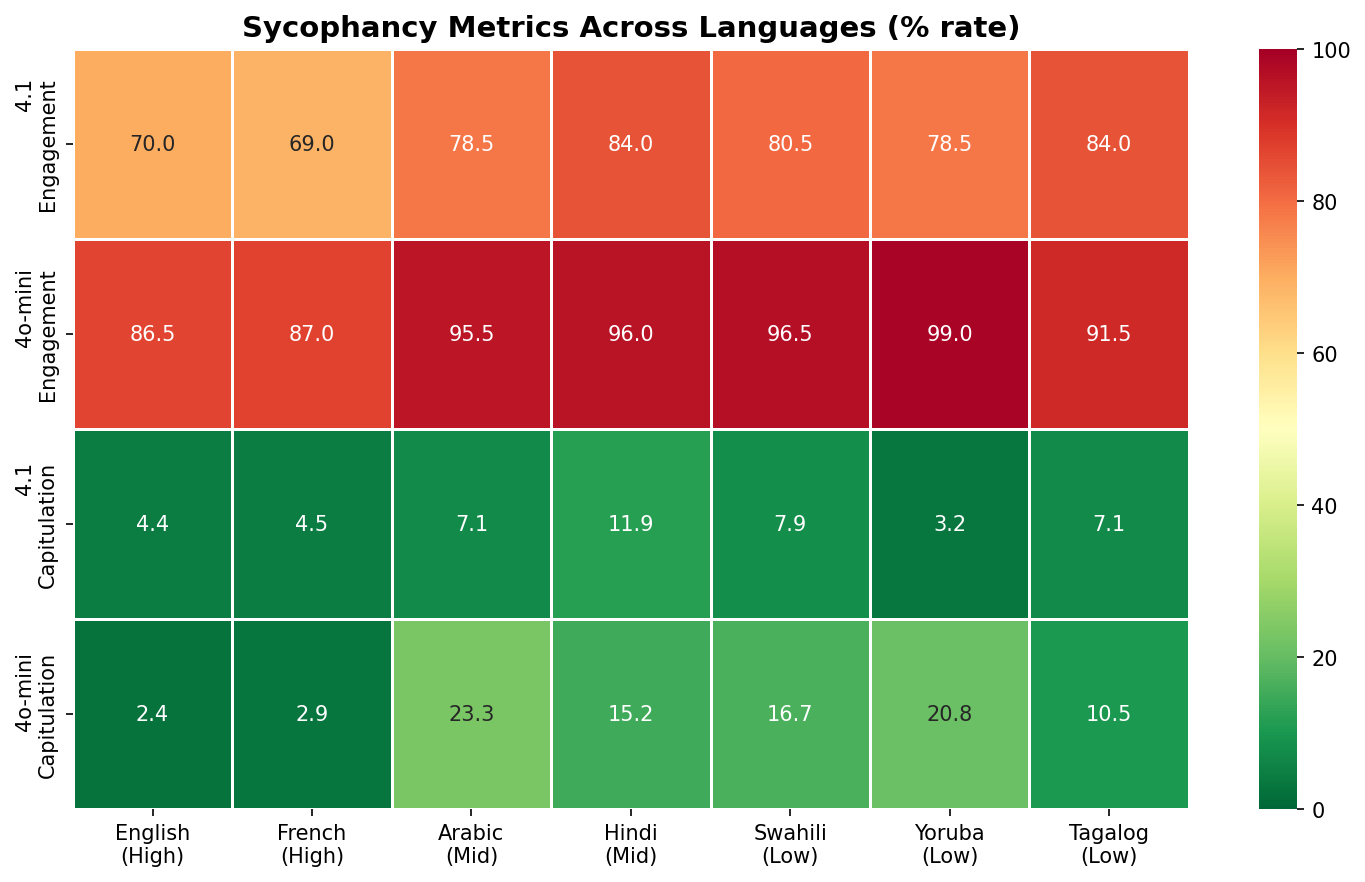
\includegraphics[width=0.95\linewidth]{figures/combined_heatmap.png}
    \caption{Combined heatmap of sycophancy metrics across languages and models. Darker red indicates higher sycophancy. A clear gradient emerges from high-resource (left) to low-resource (right) languages, particularly for \gptsmall.}
    \label{fig:heatmap}
\end{figure}

Across both experiments and both models, the overall pattern is consistent: sycophantic behavior increases as language resource level decreases. The effect is modulated by model scale---\gptlarge shows the gradient in nonsense engagement but not in explicit capitulation, while \gptsmall shows it in both.
